\section{Electroosmotic flow}\label{sec:et:electroosmosis}
Instead of driving the fluid flow through a pressure drop, a net
charged fluid may be driven by an external electric field. This may
be seen as the opposite case to that in section
\ref{sec:et:streaming_pot} where a current is induced by a pressure
drop.

The volumetric force on the fluid from the external field, $\E_{ext}$,
is given by

\begin{equation}
\F = \rhorm_e \E_{ext}
\end{equation}

where $\rho_e$ is the charge density. If the electric field is
constant (or at least has the same direction) everywhere, the sign of
the force is not in the same direction for a net charged positive area
of the fluid as for a net charged negative. Thus the fluid may be
either slowed down or sped up. This is a qualitative difference to
pressure driven situation and is illustrated in fig. \ref{fig:et:eo}.

\begin{figure}
\begin{center}
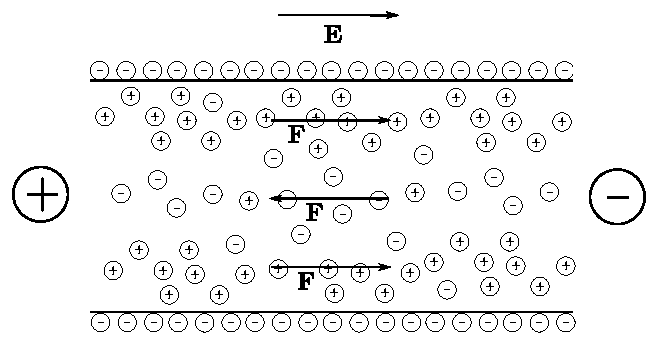
\includegraphics[width=0.7\textwidth]{fig/channel_electroosmosis.pdf}
\end{center}
\caption[Example of an electroosmotic system.]{Example of an
  electroosmotic system. The fluid is driven by an external electric
  field, $\E$. The directions of the forces on the fluid from the
  electric field are indicated with arrows. Note however that the
  fluid does not necessarily has to flow in the direction of the
  force, this due to viscous effects in the fluid. }
\label{fig:et:eo}
\end{figure}

The electroviscous effect is in the case of pure electroosmotic flow
usually neglected as the field due to the streaming potential is, in
most physical cases, small in comparison to the applied external
field. \cite{wang-poi}
